\documentclass{article}[letterpaper, 11pt]
\usepackage{geometry}
\geometry{left=1.7cm,top=2.18cm,bottom = 2.5cm,right=2.3cm}
\usepackage[utf8]{inputenc}
\usepackage{amsmath}
\usepackage{bbm}
\usepackage{amssymb}
\usepackage{enumitem}

\usepackage{lastpage}
\usepackage{fancyhdr}
\usepackage{graphicx}
\graphicspath{ {images/} }

\usepackage[parfill]{parskip}

\usepackage{color}   %May be necessary if you want to color links
\usepackage{hyperref}
\hypersetup{
    colorlinks=true, %set true if you want colored links
    linktoc=all,     %set to all if you want both sections and subsections linked
    linkcolor=black,  %choose some color if you want links to stand out
}

%Style :
\pagestyle{fancy}
\renewcommand{\thepage}{}
%commancer le compte des pages après
\setlength{\headsep}{14.5pt}

%Style nouveau chapitre
\fancyhf{}
\fancyhead[L]{\small INF2705 Infrographie}
\fancyhead[C]{\small TP3 Stencil et illumination Phong, Gouraud et Flat}
\fancyhead[R]{\small Page \thepage\hspace{1pt} sur~\pageref{LastPage}}
\fancyfoot[L]{\scriptsize Polytechnique Montréal}
\fancyfoot[C]{\scriptsize Matthieu Basset, Automne 2023}
\fancyfoot[R]{\scriptsize Département de génie informatique et génie logiciel}
\renewcommand{\headrulewidth}{0.5pt}
\renewcommand{\footrulewidth}{0.2pt}

\title{INF2705 Infrographie\\
Travail pratique 3\\
Stencil et illumination Phong, Gouraud et
Flat}
\date{Octobre 2023}
\author{Matthieu Basset}
\begin{document}

\thispagestyle{empty}
\maketitle
\newpage

\renewcommand{\thepage}{\arabic{page}}
\pagestyle{fancy}
\renewcommand{\contentsname}{Table des matières}
\setcounter{page}{1}
\tableofcontents


\newpage

\section{Introduction}
Ce document décrit les exigences du TP3 ``\textit{Stencil et illumination Phong, Gouraud et Flat}'' (Automne
2023) du cours INF2705 Infographie.
\subsection{But}
Le but des travaux pratiques est de permettre à l'étudiant de directement appliquer les notions vues
en classe.

\subsection{Portée}
Chaque travail pratique permet à l'étudiant d'aborder un sujet spécifique.

\subsection{Remise}
% chktex-file 26
Faites la commande ``\texttt{make remise}'' ou exécutez/cliquez sur ``\texttt{remise.bat}'' afin de créer l'archive \\``\textbf{ INF2705\_remise\_TPn.zip}'' (ou .7z, .rar, .tar) que vous déposerez ensuite sur Moodle (qui ajoute automatiquement vos matricules ou le numéro de votre groupe au nom du fichier remis).\\
Ce fichier \texttt{zip} contient tout le code source du TP (\texttt{makefile}, \texttt{*.h}, \texttt{*.cpp}, \texttt{*.glsl}, \texttt{*.txt}).

\newpage
\section{Description globale}
\subsection{But}

Le but de TP est de permettre à l'étudiant de mettre en pratique les concepts de stencil et d'illumination. Il sera en mesure d'effectuer des tests de stencil pour masquer certains éléments dans la scène. Il sera aussi capable de produire différents modèles d'illumination afin d'ajouter beaucoup plus de réalisme aux scènes 3d. Il sera en mesure d'implémenter différents types de source de lumière.
\\
Le travail fera l'utilisation des fonctions d'OpenGL \texttt{glStencilOp}, \texttt{glStencilFunc}, \texttt{glStencilMask} et
des \textit{shaders} de vertex, géometrie et fragment.

\subsection{Travail demandé}

Le TP3 est une continuation du TP2, cependant un projet vous est fourni. Le projet contient la solution du TP2, quelques modifications aux classes existantes et un début de projet pour vous guider dans le TP3.\vspace*{11pt}
\\
La classe \texttt{Camera} prend maintenant en argument une distance pour la caméra en troisième personne qu'on peut modifier avec le déroulement de la molette.
La classe \texttt{UniformBuffer} a été ajoutée pour faciliter l'envoi et le partage des données de lumières dans les nuanceurs.
Dans la classe \texttt{Window}, on a ajouté une méthode pour bloquer ou non la souris dans la fenêtre.
On y a aussi ajouté la gestion de la librairie IMGUI.\vspace*{11pt}
\\
Une restructuration du code a été faite pour gérer plusieurs scènes de rendu à la fois et partager les ressources entre elles.
Vous allez à partir de maintenant utiliser la classe \texttt{Resources} pour instancier les \textit{shader programs}, les modèles et les textures.
Ceux-ci seront accessible à partir de l'objet \texttt{m\_res} dans la classe \texttt{Scene}.
Au lieu de modifier la \textit{main loop} dans le \textit{main}, vous devez utiliser la méthode \texttt{Scene::render} pour générer votre affichage pour une scène en particulier.
L'ancienne scène du TP2 est disponible pour vous servir de gabarit.\vspace*{11pt}
\\
Pour le débuguage, il peut être pratique d'utiliser l'application \texttt{RenderDoc}.

\newpage
\textbf{Partie 1 : Test de stencil}\vspace{11pt}\\
On demande d'implémenter un halo coloré qui nous permettera de distinguer les singes alliés des singes ennemis dans la scène.
\begin{figure}[h]
	\begin{minipage}[c]{.49\linewidth}
		 \centering
		 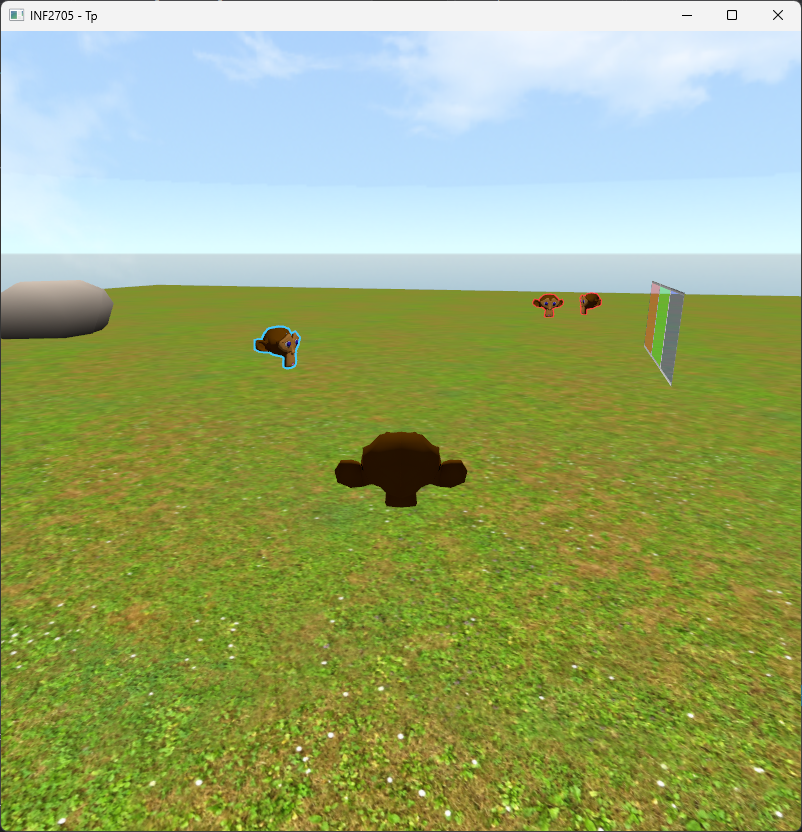
\includegraphics[scale = 0.25]{image_1.png}
	\end{minipage}
	\begin{minipage}[c]{.49\linewidth}
		 \centering
		 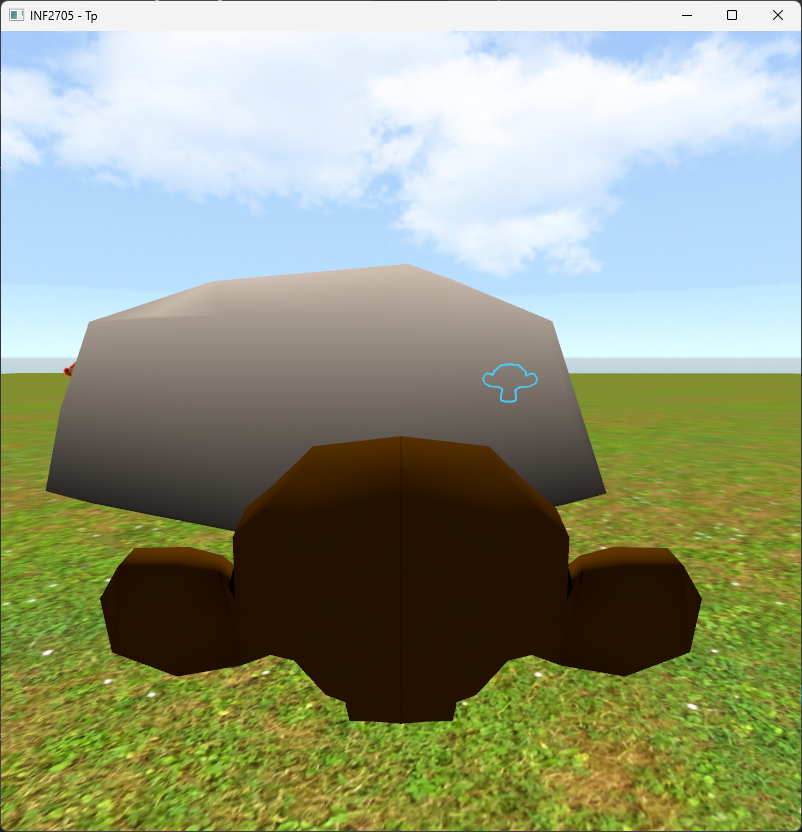
\includegraphics[scale = 0.25]{image_2.png}
	\end{minipage}
		 \caption{ \centering Effet de halo. On voit le halo bleu au travers des autres objets.}
\end{figure}\\
L'utilisation du stencil est idéale pour produire cet effet visuel. On procède généralement dans cette
ordre :
\begin{itemize}[label={--}]
	\item Dessiner l'objet avec le test de stencil pour écrire dans le tampon de stencil.
	\item Désactiver l'écriture du test de stencil.
	\item Modifier le test pour réussir seulement aux endroits où l'objet n'est pas présent.
	\item Dessiner l'objet plus gros (halo) avec un \textit{shader} simple d'une seule couleur.
\end{itemize}

Pour ce faire, vous devez activer le test de stencil lors du dessin des singes alliés et ennemis.
Leurs \textit{draw} \textit{calls} devront en tout temps écrire dans le stencil pour pouvoir définir leur contour.
Pour chaque singe que vous dessinez, utilisez et modifiez un bit différent pour pouvoir les différencier (utiliser \texttt{glStencilMask} pour permettre l'édition seulement sur les bits spécifiés).\vspace*{11pt}
\\
Les singes et leurs halo auront la même position. Il est recommandé de précalculer la matrice mvp
une seule fois pour l'utiliser avec les modèles et les halos. Par la suite, on dessinera les halos avec
un shader simple.\vspace*{11pt}
\\
Le \textit{vertex shader} prendra en entrée la position et la normale du vertex et n'aura aucune sortie (autre que \texttt{gl\_Position}). Il nous faudra l'attribut de normale des modèles 3d. Celui-ci est activable de la même façon que lors du TP2 dans le chargement des données (déjà réalisé). Pour agrandir l'objet, une simple mise à l'échelle donnerait un effet inconstant, d'autant plus que l'origine de l'objet n'est pas au centre du modèle. On préfèrera déplacerer les vertices dans la direction de leur normale d'un facteur constant.
\\
Ce facteur définira l'épaisseur de notre halo. Dans notre cas, une valeur de $0.1$ est suffisante. N'oubliez pas de normaliser votre normale !\vspace*{11pt}
\\
Le \textit{fragment shader} prendra un \texttt{uniform vec3} de la couleur pour définir la couleur de sortie. Celle-ci définit la couleur du halo et devra être envoyée avant de dessiner l'objet.\vspace*{11pt}
\\
Pour dessiner les halos, il faudra désactiver l'écriture du test de stencil. Le test doit passer lorsque le bit du singe traité est à 0 (où il n'est pas présent).\vspace*{11pt}
\\
Pour le singe allié, on veut qu'il soit toujours visible au travers des autres objets. Vous allez devoir
modifier la fonction du test de profondeur pour y parvenir.
\vspace*{11pt}
\\
Vous ne devez pas faire plusieurs appels à \texttt{glClear}.\vspace*{11pt}
\\
De plus, on dessinera un mur de vitres colorées. On appliquera le test de \textit{blending} pour pouvoir faire le mélange de couleur avec la scène. Le facteur source sera l'alpha source $(\alpha_{src})$ et le facteur destination sera un moins l'alpha source $(1-\alpha_{src})$.
Le mur doit être visible des deux sen1s. N'oubliez pas d'utiliser alpha dans le \texttt{fragColor} finale.

\begin{figure}[h]
		 \centering
		 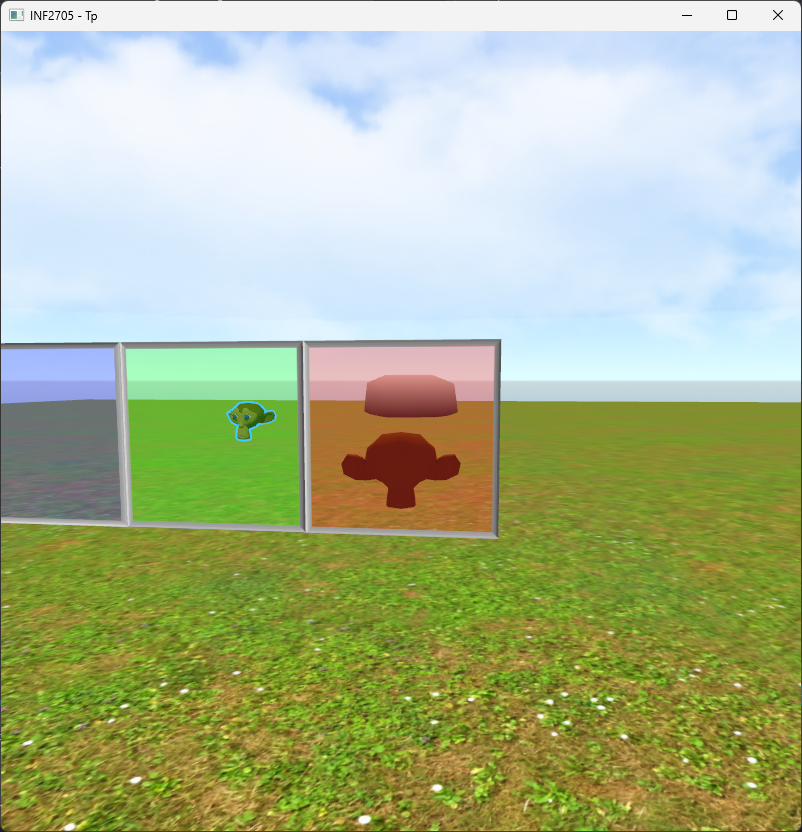
\includegraphics[scale = 0.30]{image_3.png}

		 \caption{ \centering \textit{Blending}}
\end{figure}

\newpage
\textbf{Partie 2 : Illumination}\vspace{11pt}
\\
Même avec l'ajout des textures, la scène manque de réalisme. Pour remédier à ce problème, l'ajout
d'illumination va permettre de grandement améliorer le rendu.

\begin{figure}[h]
	\begin{minipage}[c]{.33\linewidth}
		 \centering
		 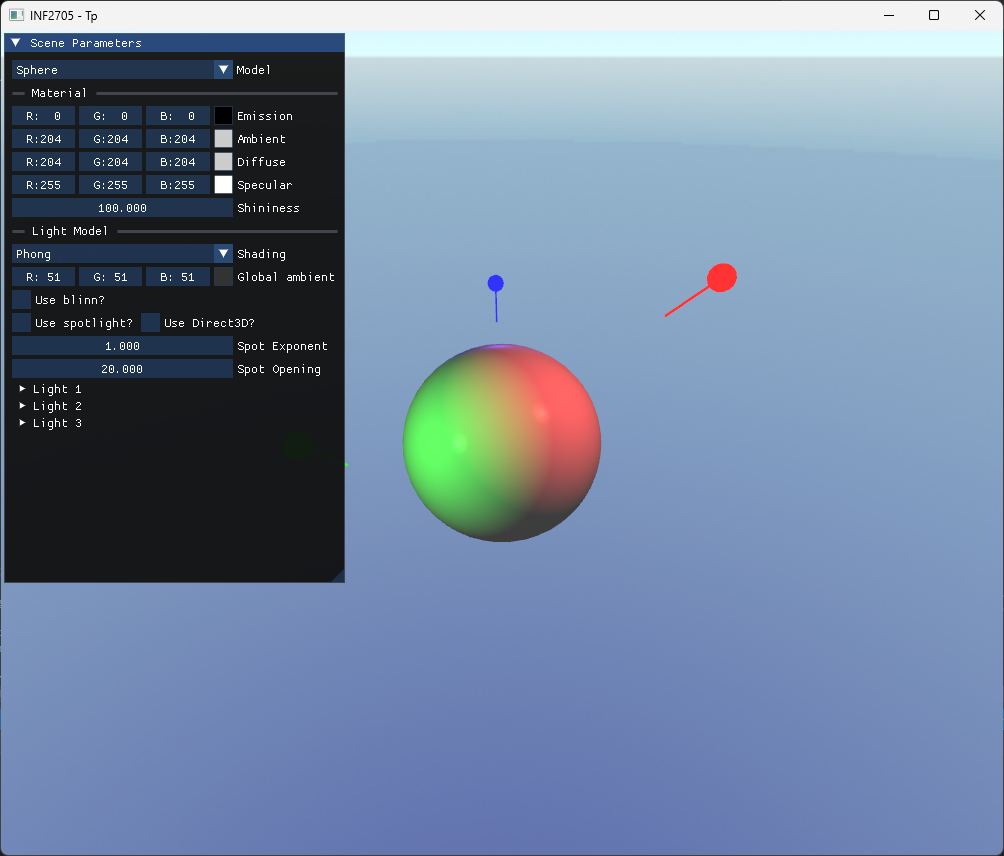
\includegraphics[scale = 0.15]{image_4.png}
	\end{minipage}
	\begin{minipage}[c]{.33\linewidth}
		 \centering
		 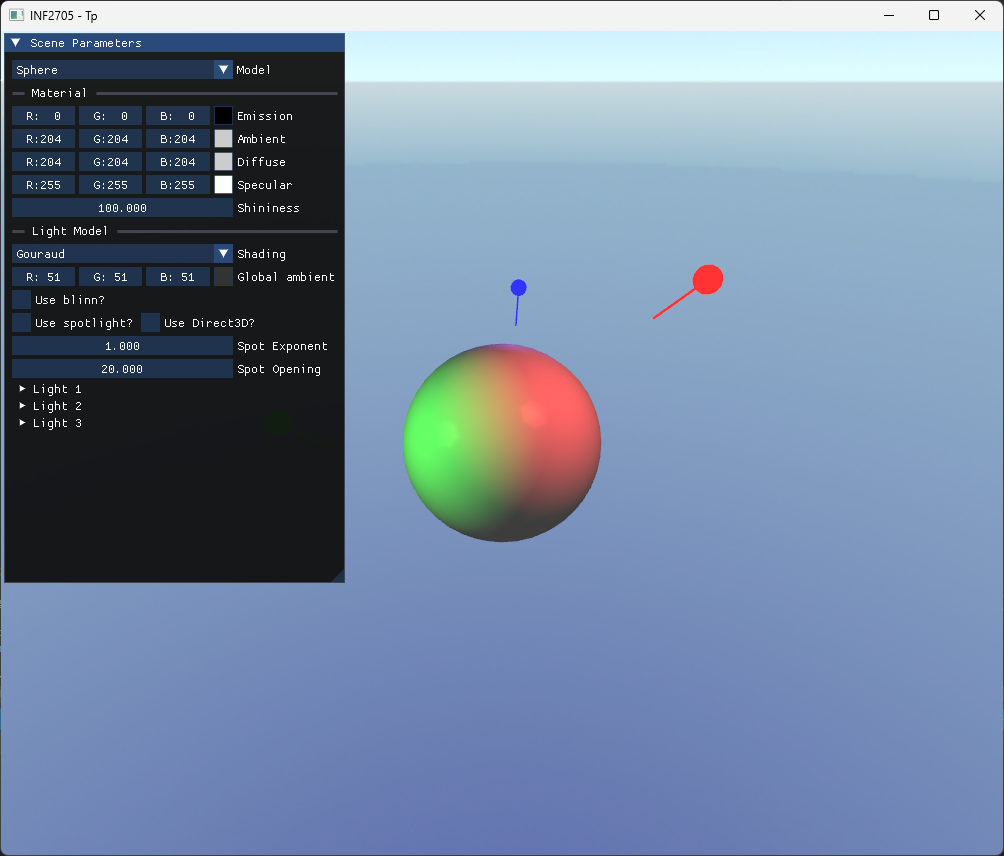
\includegraphics[scale = 0.15]{image_5.png}
	\end{minipage}
	\begin{minipage}[c]{.33\linewidth}
		\centering
		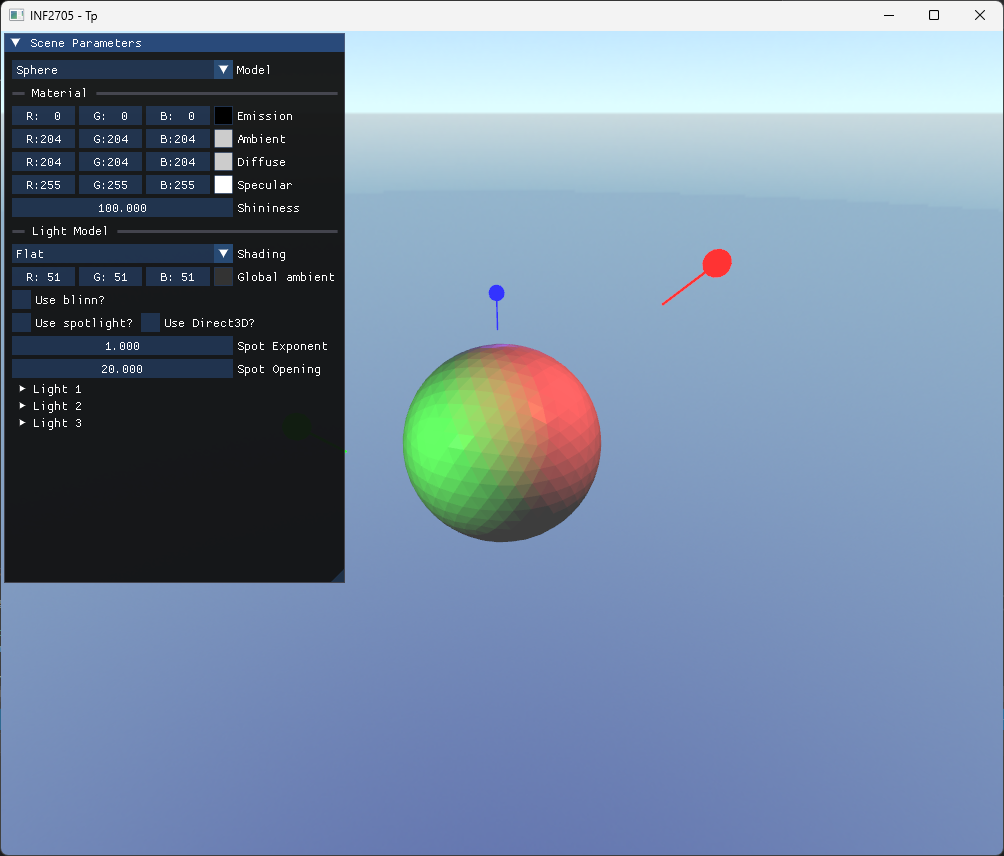
\includegraphics[scale = 0.15]{image_6.png}
  \end{minipage}
		 \caption{ \centering Illumination de Phong, Gouraud et Flat.}
\end{figure}

Une scène de developpement vous est fournie afin d'être en mesure de mieux observer le comportement de l'illumination.
Celle-ci permet d'afficher un modèle qui sera éclairé par 3 lumières. Un affichage fait avec la librairie IMGUI permet de facilement modifier les variables qui impactent le modèle d'illumination.\vspace*{11pt}
\\
La majeure partie du code C++ a déjà été réalisée pour vous économiser du temps. Celui-ci s'occupe de la gestion du \textit{uniform buffer}, gère le changement de \textit{shader}, de modèle et le dessin des sources de lumière.\vspace*{11pt}
\\
Pour cette partie, vous allez faire les modifications directement dans les \textit{shaders}. On demande de faire le calcul d'illumination des sources de lumière positionnelles, sans le facteur d'atténuation.
Vous devez implémenter les modèles d'illumination de Phong, Gouraud et Flat. Il est recommandé de se baser sur les exemples vus en cours.\vspace*{11pt}
\\
Voici quelques directives supplémentaires pour vous aider :
\begin{itemize}[label={--}]
	\item Un début de déclaration de \textit{shader} a été fait pour chaque modèle.
	\item On utilise un \textit{interface block} pour permettre de mieux nommer les \texttt{in} et \texttt{out} des \textit{shaders}.
	Seulement les noms de blocs ont besoin d'être identiques entre les \textit{shaders}, le nom de la variable peut changer.
	\item Le bloc uniforme \textit{LightingBlock} est défini pour contenir les données d'illumination. Vous ne devriez pas changer cette structure de données, au risque d'avoir des mauvais \textit{offsets} de mémoire.
	\item Le code de l'illumination est sensiblement le même dans les trois \textit{shaders}. Vous allez malheureusement être obligés de dupliquer le code dans les 3.
	\item Les calculs devront être fait dans le référentiel de la caméra.
	\item Faites la normalisation des vecteurs après la rastérisation pour les attributs utilisé dans le \textit{fragment shader}.
	\item N'oubliez pas d'appliquer la matrice de normale.
	\item Vous devez implémenter la réflexion spéculaire de Blinn et de Phong.
	\item Vous devez implémenter le calcul des \textit{spotlights} avec le calcul d'OpenGL classique et le calcul de Direct3d.
\end{itemize}

\begin{figure}[ht]
	\begin{minipage}[r]{.49\linewidth}
		 \begin{flushright}
			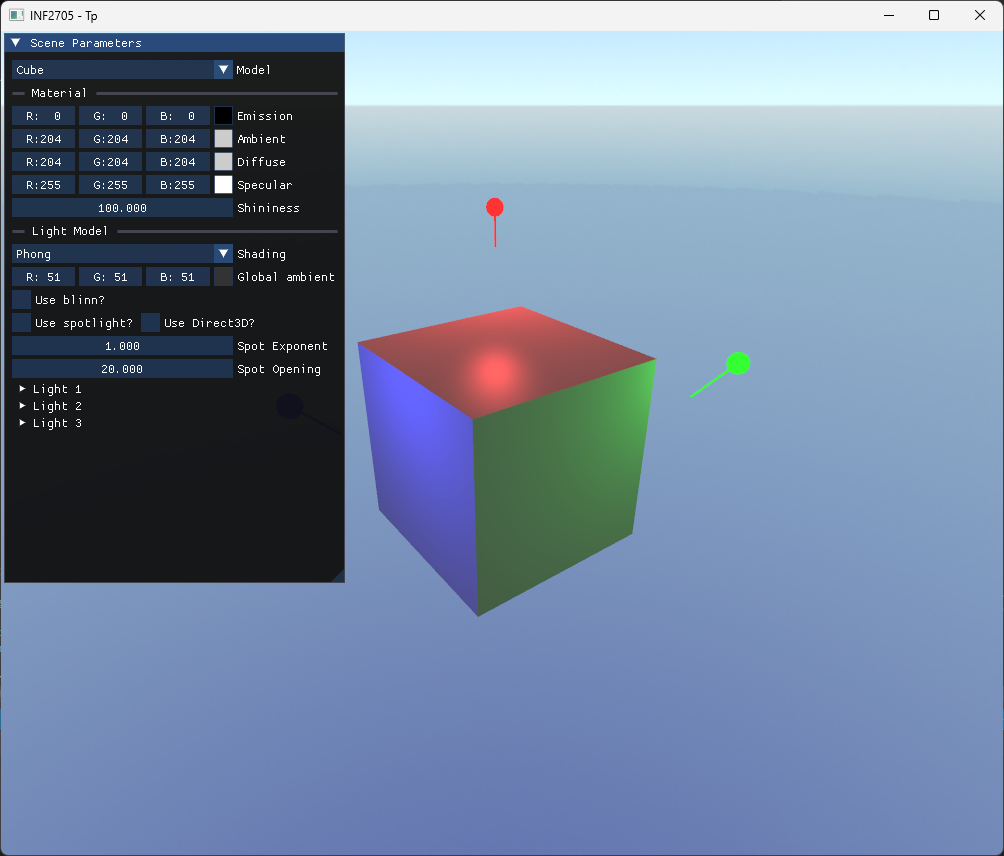
\includegraphics[scale = 0.16]{image_7.png}
		 \end{flushright}
	\end{minipage}
	\begin{minipage}[l]{.49\linewidth}
		 \begin{flushleft}
			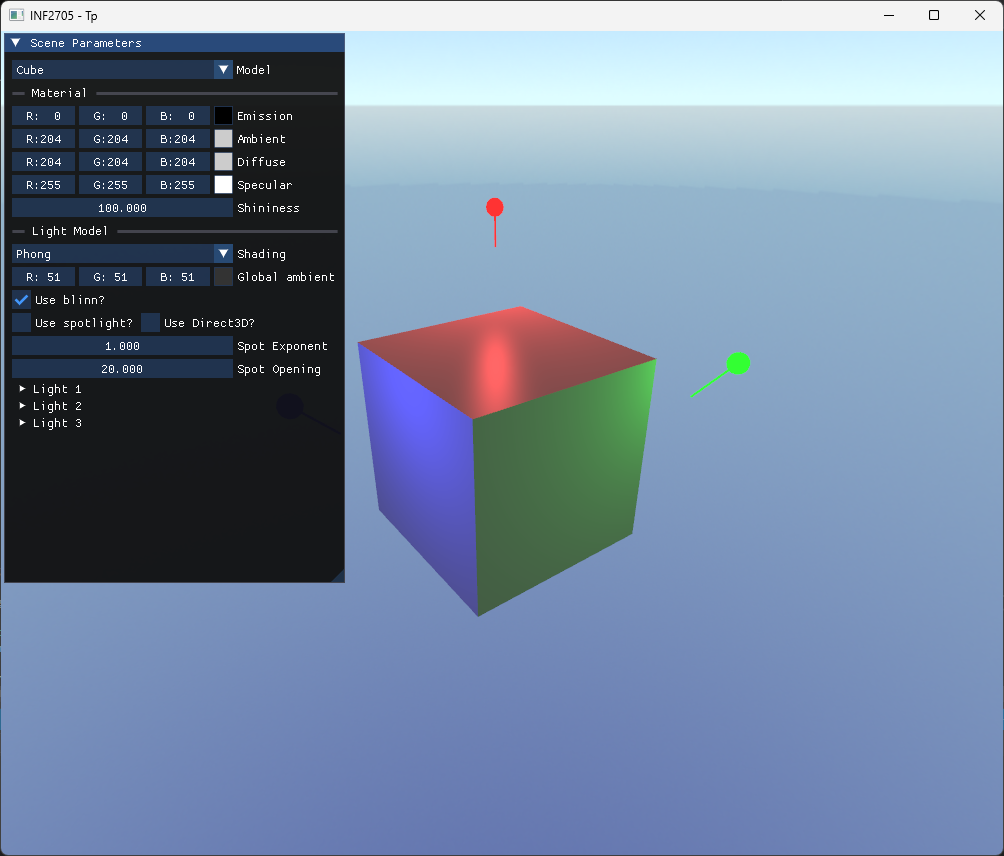
\includegraphics[scale = 0.16]{image_8.png}
		 \end{flushleft}
	\end{minipage}
		 \caption{ \centering Illumination de Phong, Gouraud et Flat.}
\end{figure}

\begin{figure}[ht]
	\begin{minipage}[c]{.33\linewidth}
		 \centering
		 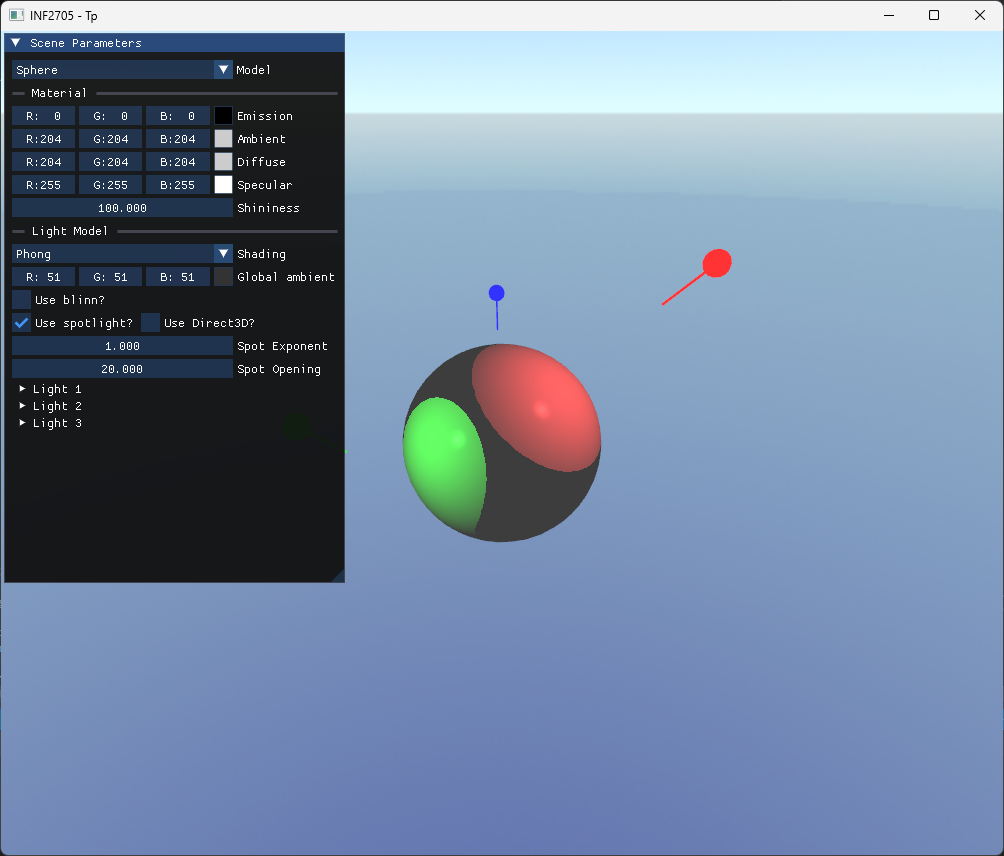
\includegraphics[scale = 0.16]{image_9.png}
	\end{minipage}
	\begin{minipage}[c]{.33\linewidth}
		 \centering
		 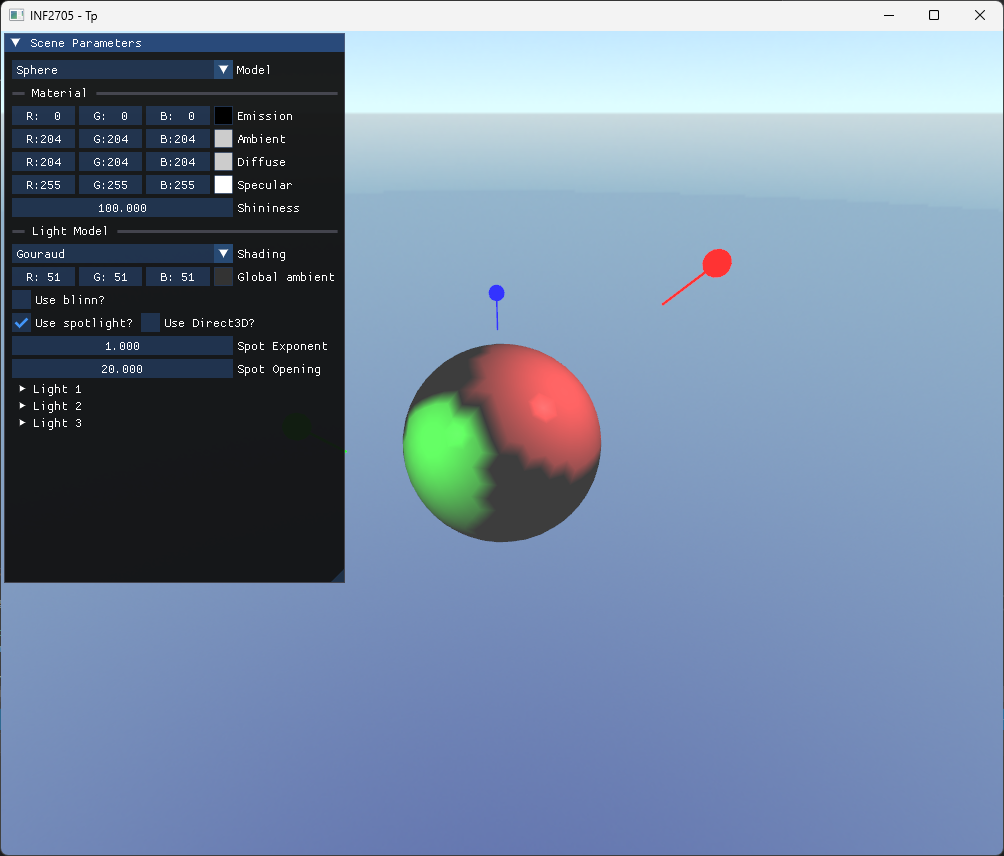
\includegraphics[scale = 0.16]{image_10.png}
	\end{minipage}
	\begin{minipage}[c]{.33\linewidth}
		\centering
		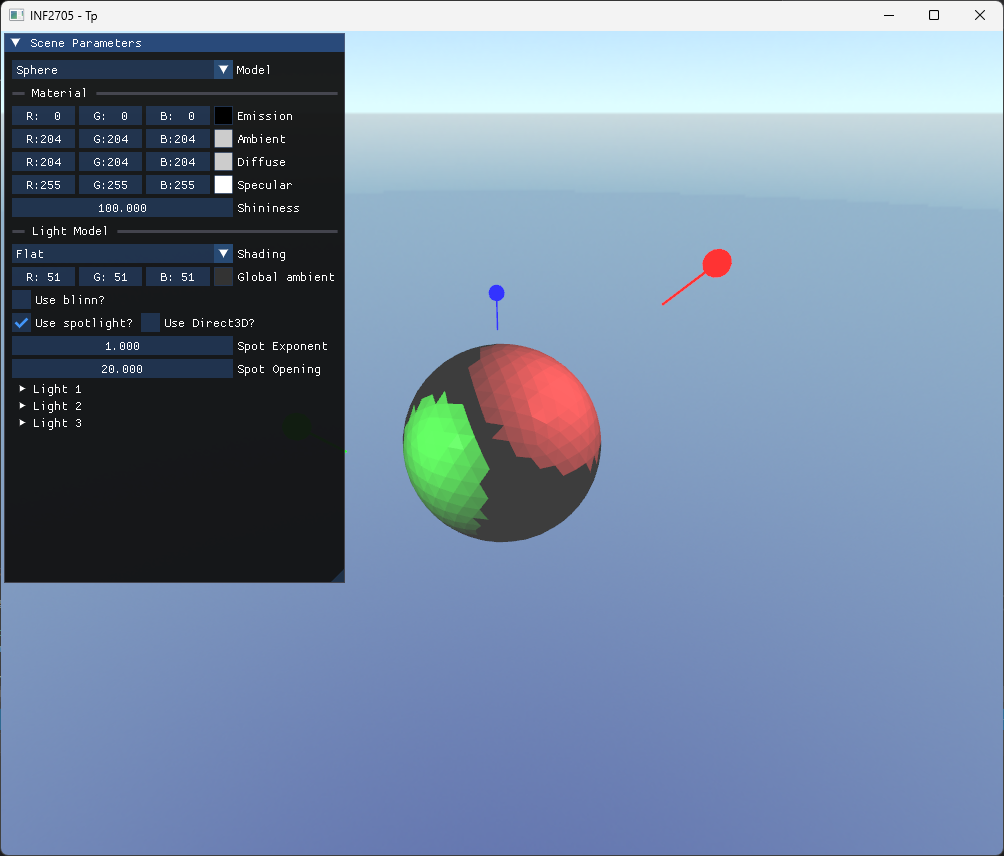
\includegraphics[scale = 0.16]{image_11.png}
  \end{minipage}
		 \caption{ \centering Spotlight de Phong, Gouraud et Flat avec l'algorithme d'OpenGL classique.}
\end{figure}

Pour l'illumination Flat, on a besoin de calculer l'illumination par face. Le \textit{vertex shader} calculera la position finale transformée par \texttt{mvp} et envoit les autres attributs tels quels. On aura un \textit{shader} de géometrie pour faire le calcul d'illumination. Celui-ci calculera la normale par face de la façon suivante :\\
% chktex-file 8
% chktex-file 36
\texttt{vec3 side1 = (Vertex1 - Vertex0);}\\
\texttt{vec3 side2 = (Vertex2 - Vertex0);}\\
\texttt{normal = cross(side1, side2);}\vspace*{11pt}
\\\newpage
La position est le centre de la face du triangle. Vous devez calculer la position du centre. Les calculs d'illumination ne devraient être fait qu'une seule fois pour chaque face traitée.\vspace*{11pt}
\\
%chktex-file 44
Il est recommandé de commencer par l'illumination de Phong avec une seule lumière. Par la suite, on peut facilement appliquer la même logique pour les autres modèles d'illumination. Certaines formules sont expliqués davantage dans la section~\ref{sec:formules} et les notes de cours.

\begin{figure}[h]
	\begin{minipage}[c]{.33\linewidth}
		 \centering
		 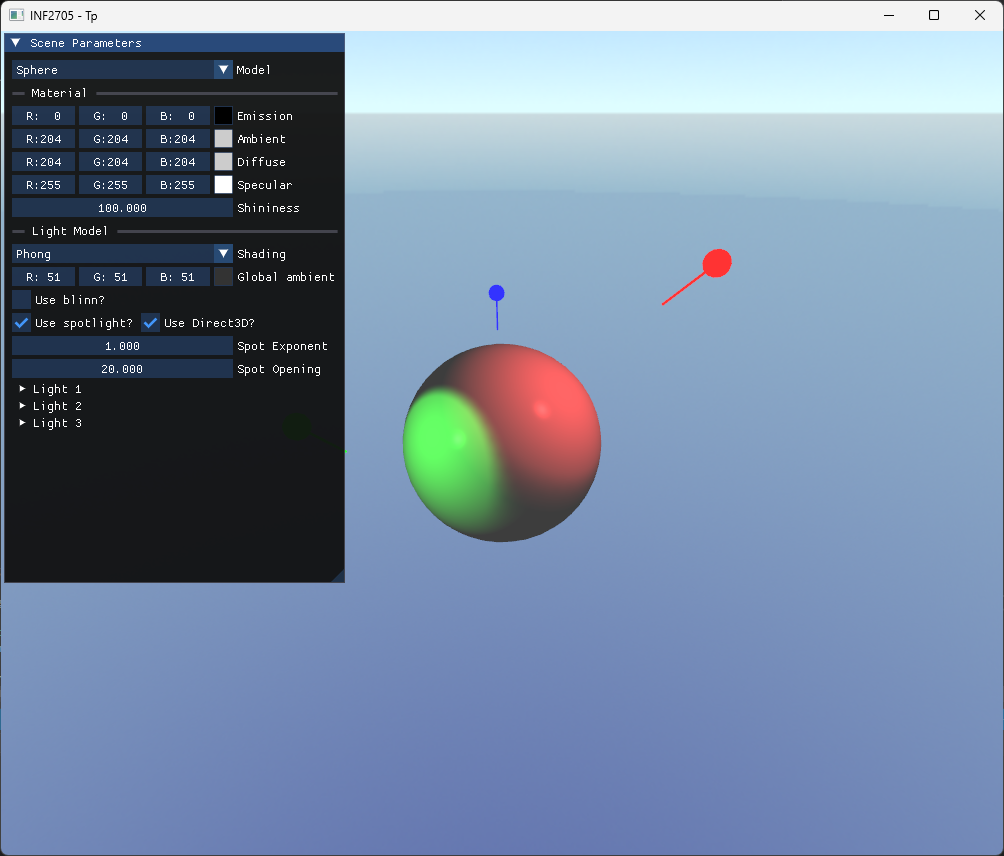
\includegraphics[scale = 0.16]{image_12.png}
	\end{minipage}
	\begin{minipage}[c]{.33\linewidth}
		 \centering
		 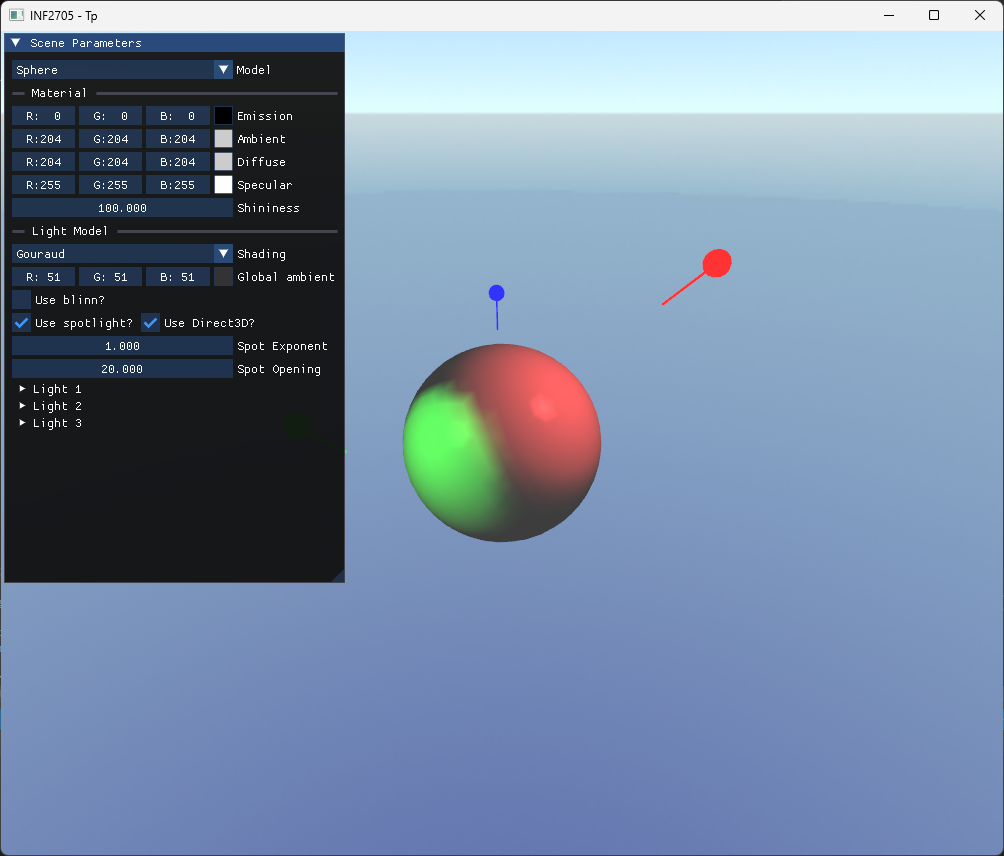
\includegraphics[scale = 0.16]{image_13.png}
	\end{minipage}
	\begin{minipage}[c]{.33\linewidth}
		\centering
		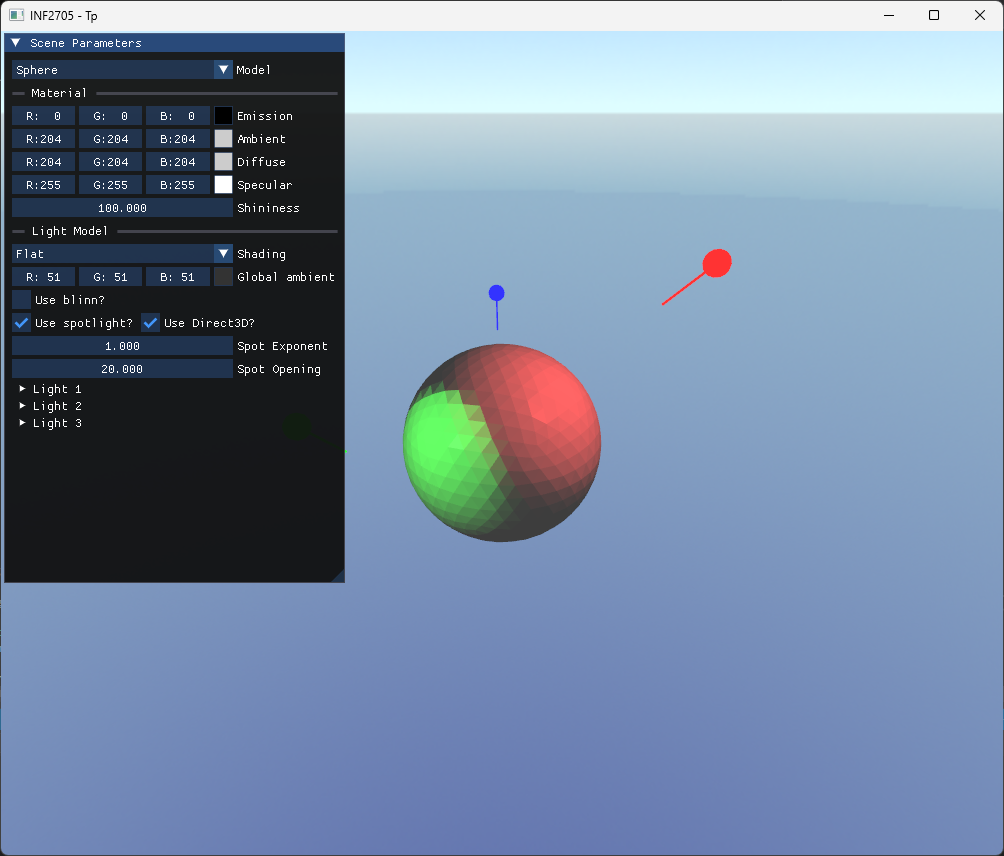
\includegraphics[scale = 0.16]{image_14.png}
  \end{minipage}
		 \caption{ \centering Spotlight de Phong, Gouraud et Flat avec l'algorithme de DirectDraw.}
\end{figure}

Avec l'llumination de Phong, on va pouvoir utiliser des textures pour paramétrer notre illumination.
La couleur de la texture diffuse devrait seulement être prise en compte dans le facteur ambiant et diffus de l'illumination. Garder le \textit{alpha discard} (si alpha $< 0.3$).
La texture spéculaire sera appliquée sur le facteur spéculaire pour pouvoir appliquer des reflets à des endroits spécifiques.
Prenez note que c'est une texture à une seule composante. Vous allez vouloir diviser ou modifier la fonction \texttt{computeLight} en deux pour séparer la composante diffuse de la composante spéculaire.\vspace*{11pt}
\\
Notez que la texture spéculaire est en teinte de gris (d'où la raison d'avoir une seule composante), principalement parce que la couleur spéculaire est dans la majorité des cas définie par la source de lumière plutôt que par le matériau. Seulement l'intensité nous intéresse ici.\vspace*{11pt}
\\
Pour Gouraud, on envoit les quatres composantes (emission, ambiant, diffuse et spéculaire) séparées au \textit{fragment shader}.
Le \textit{fragment shader} pourra les recomposer et appliquer les textures sur les bonnes composantes.
\begin{figure}[h]
	\begin{minipage}[c]{.49\linewidth}
		 \centering
		 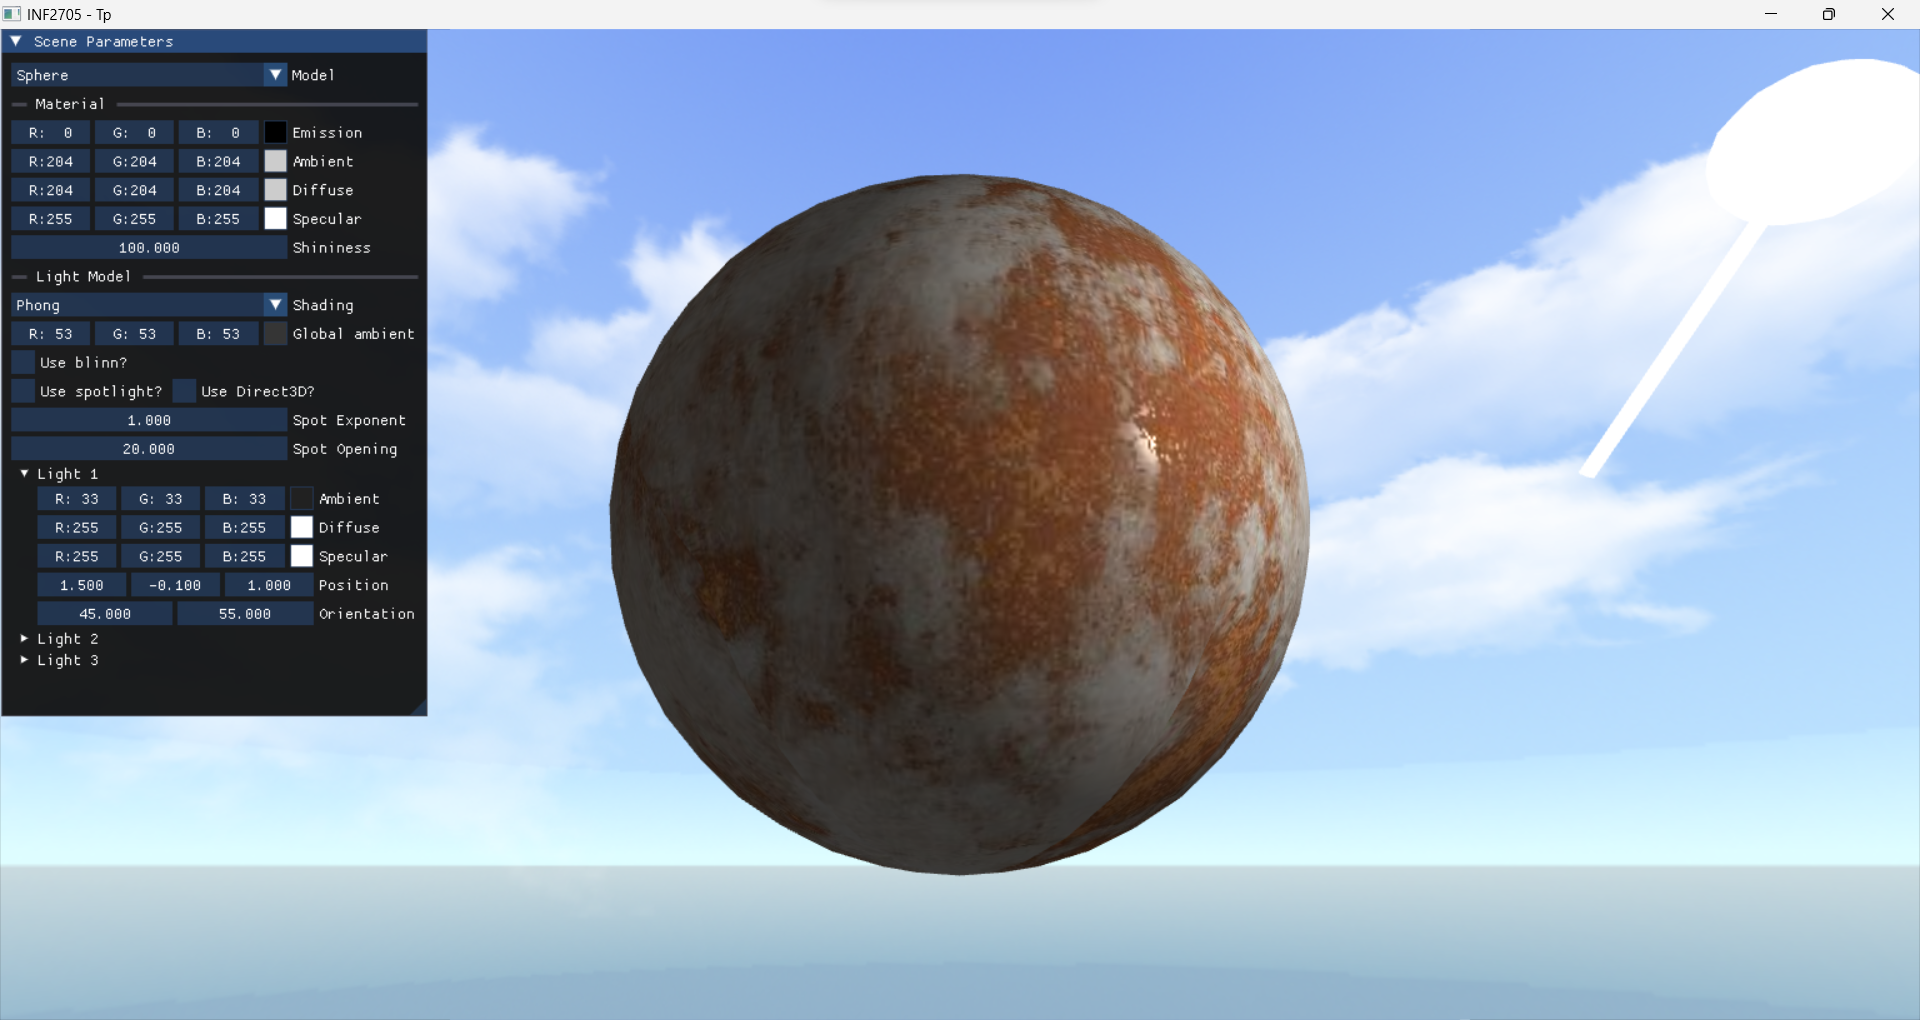
\includegraphics[scale = 0.125]{image_15.png}
	\end{minipage}
	\begin{minipage}[c]{.49\linewidth}
		 \centering
		 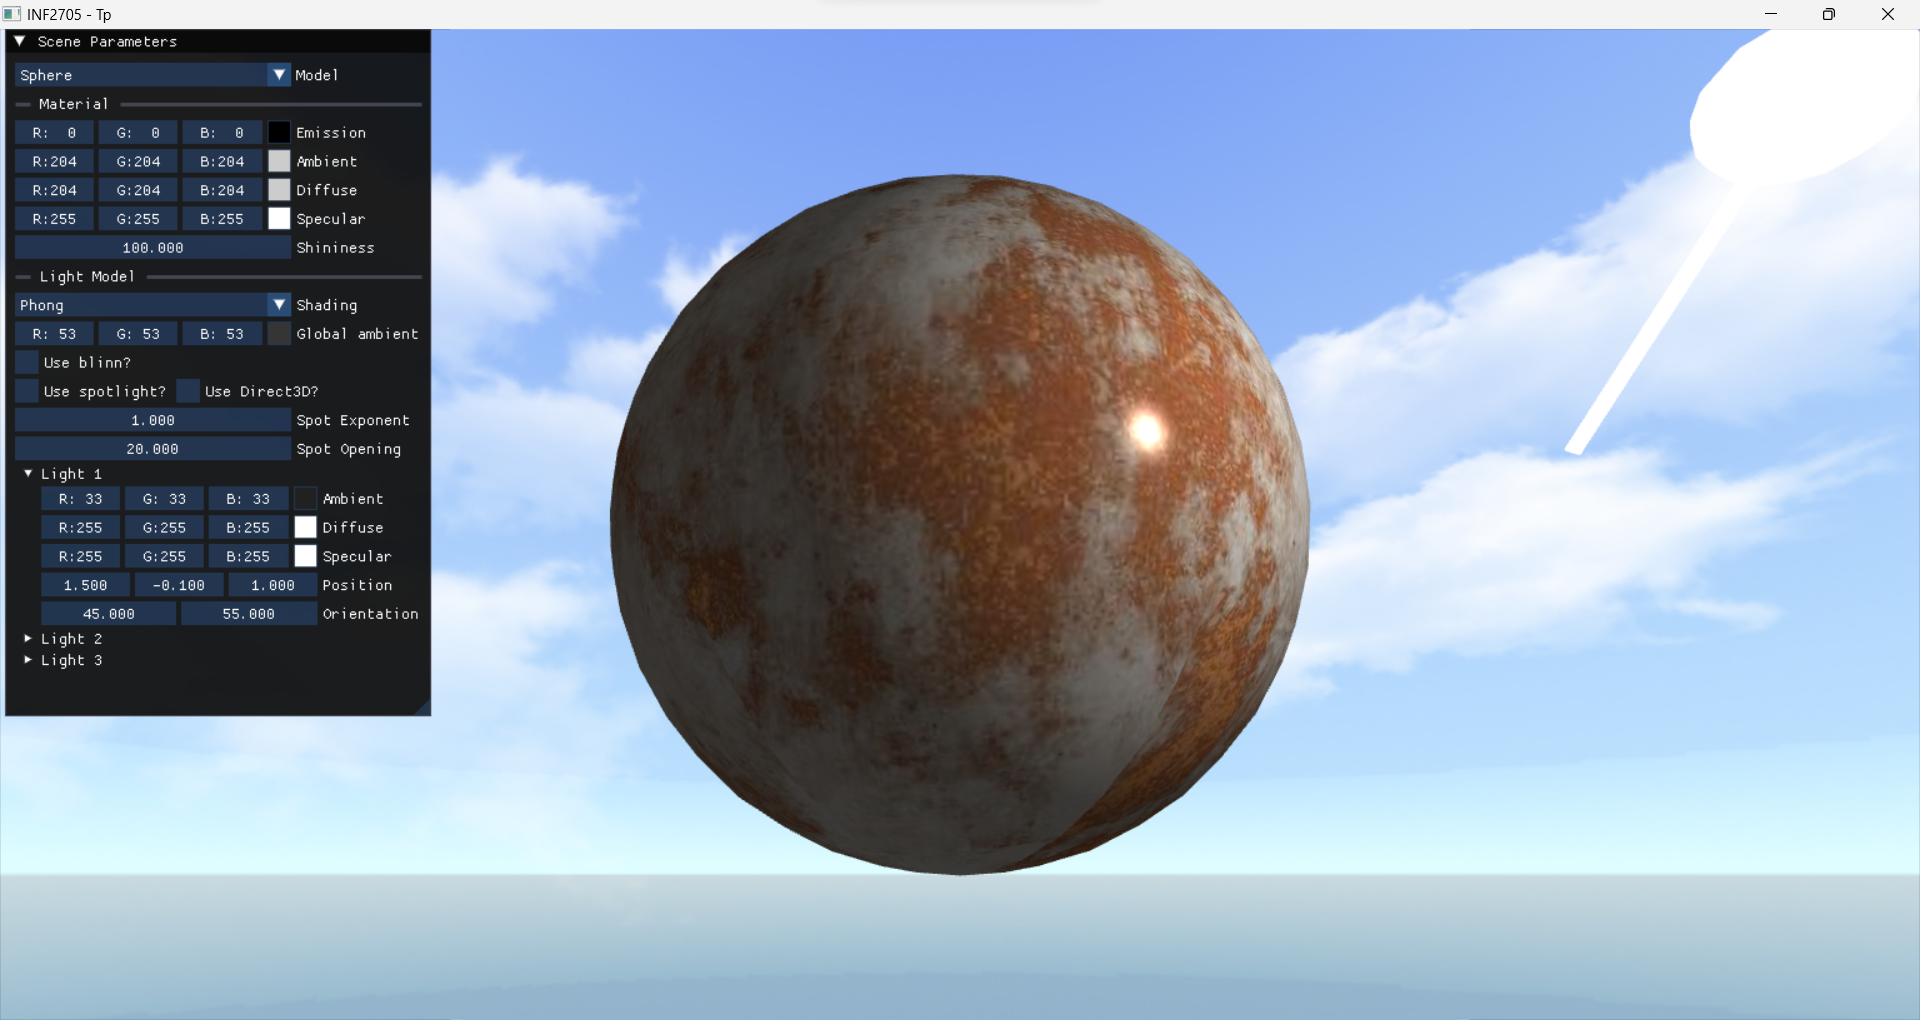
\includegraphics[scale = 0.125]{image_16.png}
	\end{minipage}
		 \caption{ \centering Comparaison avec et sans \textit{lightmaps} appliqués sur la sphère avec l'illumination de Phong.}
\end{figure}

Suite à la réalisation des \textit{shaders} d'illumination, on pourrait éclairer notre scène du TP précédent. Cependant, pour vous économisez du travail redondant, cette scène vous sera donnée lors du prochain TP.\@

\newpage
\section{Exigences}
\subsection{Exigences fonctionnelles}
\underline{Partie 1:}
\begin{enumerate}[label={E\arabic*.}]
	\item  Les matrices \texttt{mvp} sont précalculées pour les singes. [1 pt]
	\item Le \textit{shader} simple agrandit la géométrie et colorie celle-ci correctement. [1 pt]
	\item Les paramètres de stencil sont corrects et permettent de modifier seulement le bit voulu. [1 pt]
	\item Le stencil est modifié seulement lors du dessin des singes (les halos ne l'écrivent pas). [1 pt]
	\item La halo est seulement impacté par le stencil écrit par le singe correspondant (le masque est correct). [1 pt]
	\item Les halos des singes ennemis ne sont visibles que lorsqu'il n'y a aucun obstacle entre la vue et le singe. [1 pt]
	\item Le halo du singe allié est visible en permanence au travers des autres objets. [2 pts]
	\item Aucun \texttt{glClear} supplémentaire n'est utilisé. [1 pt]
	\item Les tests de stencil et \textit{blending} sont activés seulement pour le dessin des fragments consernés. [2 pts]
	\item Les paramètres de \textit{blending} sont corrects pour voir au travers de façon à teindre la vue. [2 pts]
	\item Les halos sont visibles au travers de la vitre (et du contour de celle-ci, malheureusement).
	[1 pt]
	\item Le mur est visible des deux côtés lorsqu'on le regarde. [1 pt]
\end{enumerate}

\underline{Partie 2:}

\begin{enumerate}[label={E\arabic*.}, resume]
	\item Le modèle d'illumination de Phong est implémenté correctement. [5 pts]
	\item Le modèle d'illumination de Gouraud est implémenté correctement. [5 pts]
	\item Le modèle d'illumination de Flat est implémenté correctement avec un \textit{shader} de géométrie. [5 pts]
	\item Les réflexions spéculaires de Blinn et Phong sont implémentées correctement. [2 pts]
	\item Les spotlights sont implémentées correctement avec la version d'OpenGL et Direct3D dans les 3 \textit{shaders}. [5 pts]
	\item Les calculs sont effectués dans le référenciel de la caméra. [1 pt]
	\item Les normalisations sont effectuées après la rasterisation plutôt qu'avant celle-ci. [1 pt]
	\item Les propriété du matériau sont utilisées correctement. [2 pts]
	\item Les textures de \textit{lightmaps} diffuse et spéculaire sont utilisées correctement pour les 3 \textit{shaders}. [3 pts]
	\item Les textures de \textit{lightmaps} n'impactent pas les propriétés du matériau. [1 pt]
\end{enumerate}

\subsection{Exigences non fonctionnelles}
De façon générale, le code que vous ajouterez sera de bonne qualité. Évitez les énoncés superflus
(qui montrent que vous ne comprenez pas bien ce que vous faites !), les commentaires erronés ou
simplement absents, les mauvaises indentations, etc. [2 pts]

\newpage
\section*{ANNEXES}

\setcounter{section}{0}
\renewcommand{\thesection}{\Alph{section}}
\section{Liste des commandes}
\begin{tabular}{ll}
\textbf{Touche} & \textbf{Description} \\
\texttt{ESC} 		& Quitter l'application \\
\texttt{w} 			& Mouvement avant \\
\texttt{s} 			& Mouvement arrière \\
\texttt{a} 			& Mouvement gauche \\
\texttt{d} 			& Mouvement droit \\
\texttt{scroll} 	& Alterner entre FPS/TPS \\
\texttt{souris} 	& Changer l'orientation de la camera \\
\texttt{espace} 	& Activer/desactiver la souris \\
\texttt{t} 			& Changer de scène \\
\textit{Ajoutées} &\\
\texttt{q}			& Descendre \\
\texttt{e}			& Monter \\
\texttt{Shift}		& Sprint \\
\end{tabular}

\newpage
\section{Formules utilisées}\label{sec:formules}
\subsection{Modèles de réflexion spéculaire de Phong et de Blinn}

Le calcul de la réflexion spéculaire fait intervenir un produit scalaire entre deux vecteurs. La différence entre les modèles de Phong et de Blinn réside dans le choix des deux vecteurs utilisés :
\begin{itemize}[label={--}]
	\item Phong utilise : $\vec{R} \cdot \vec{O} = \texttt{reflect}(-\vec{L}, \vec{N}) \cdot \vec{O}$
	\item Blinn utilise : $\vec{B} \cdot \vec{N} = \textit{\texttt{bissectrice}}(\vec{L}, \vec{O}) \cdot \vec{N} = \texttt{normalise}(\vec{L} + \vec{O}) \cdot \vec{N}$
\end{itemize}
où :\\
\begin{tabular}{lll}
	$\vec{N}$: & normale à la surface & \\
	$\vec{L}$: & direction du point vers la source lumineuse & \\
	$\vec{R}$: & direction du rayon réfléchi & $= \texttt{reflect}(-\vec{L}, \vec{N})$, avec $\vec{L}$ et $\vec{N}$ unitaires. \\
	$\vec{O}$: & direction du point vers l'observateur & \\
	$\vec{B}$: & bissectrice entre les vecteurs $\vec{L}$ et $\vec{O}$ & $= \texttt{normalise}(\vec{L} + \vec{O})$, avec $\vec{L}$ et $\vec{O}$ unitaires. \\
\end{tabular}

Tous les calculs d'illumination se font dans le repère de la caméra en GLSL.\vspace*{11pt}
\\
-- Le calcul de la direction vers l'observateur $(\vec{O})$ : (un vecteur qui pointe vers le $(0,0,0)$, c'est-à-dire vers la caméra)\\
\texttt{attribIn.obsPos = (-pos); // =(0 - pos)}\vspace*{11pt}\\
-- La direction de la lumière $(\vec{L})$ :\\
\texttt{attribIn.lumiDir[i] = (view * lights[i].position).xyz - pos;}

\newpage
\subsection{Modèles de spot inspirés d'OpenGL ou de Direct3D}

Un spot n'éclaire qu'à l'intérieur d'un cône, c'est-à-dire qu'il n'a une influence que si l'angle $\gamma$ entre la direction du spot et la direction vers le point à éclairer est plus petit que l'angle d'ouverture $\delta$ du spot.
Lorsque c'est le cas, on a `` $\gamma < \delta$ '' et mais on vérifiera plutôt si `` $\cos(\gamma) > \cos(\delta)$'' en évaluant des produits scalaires entre les vecteurs appropriés.\vspace*{11pt}
\\
Pour déterminer la direction du spot dans le repère de la caméra, on peut calculer ce vecteur de direction
directement dans le nuanceur :\vspace*{11pt}
\\
\texttt{attribIn.spotDir[i] = mat3(view) * -lights[i].spotDirection;}\vspace*{11pt}
\\
La différence entre les modèles inspirés d'OpenGL et de Direct3D que nous utiliserons réside dans la formule pour calculer le facteur qui multiplie l'intensité lumineuse du spot à l'intérieur du cône :\vspace*{11pt}
\\
-- OpenGL utilise le facteur : $\text{fact} = {(\cos \gamma)}^{c}$\vspace*{11pt}
\\
-- Direct3D utilise le facteur : $\text{fact} = \texttt{smoothstep}(\cos(\theta_{\text{outer}}), \cos(\theta_{\text{inner}}), \cos(\gamma))$

où :\\
\begin{tabular}{lll}
	$\cos \delta$ : & cosinus de l'angle d'ouverture du spot & \texttt{= cos(LightSource.spotAngleOuverture)}\\

	$\vec{L}_n$ : & direction du spot & \texttt{= LightSource.spotDirection[j]}\\

	$c$ : & exposant du spot & \texttt{= LightSource.spotExponent}\\

	$\cos \gamma$ : & est obtenu par & $\vec{L} \cdot \vec{L}_n$ \\

	$\cos \theta_{\text{inner}}$ : & est remplacé dans ce TP par & $\cos \delta$\\

	$\cos \theta_{\text{outer}}$ : & est remplacé dans ce TP par & ${(\cos \delta)}^{1.01 + c/2}$\\

\end{tabular}
\end{document}
